\documentclass{article}
\usepackage{amsmath, sfmath, multicol, tkz-euclide, array, enumerate, tcolorbox, tabularray}
\renewcommand{\familydefault}{\sfdefault}
\setlength{\parindent}{0cm}
\pagestyle{empty}
\usepackage[left=1in, top=0.5in, right=1in, bottom=0.5in]{geometry}
\tikzset{>=stealth}
\tcbset{colback=white}

\newcounter{example}[section]
\newenvironment{example}[1][]{\refstepcounter{example}\par\medskip
   {\color{red}\textbf{Example~\theexample. #1}}}{\medskip}

\begin{document}

\section*{Corresponding Parts of Congruent Triangles are Congruent (CPCTC)}

\begin{tcolorbox}[colframe=orange!70!white, coltitle=black, title=\textbf{Today I Can}]
\begin{enumerate}
    \item Use triangle congruence and corresponding parts of congruent triangles to prove that parts of two triangles are congruent.
\end{enumerate}
\end{tcolorbox}
\bigskip 

Recall that if triangles are congruent, then all corresponding parts (sides and angles) are congruent. This can be summarized as follows:
\begin{center}
Corresponding Parts of Congruent Triangles are Congruent (CPCTC)
\end{center}

Steps to Using CPCTC:
\begin{enumerate}
    \item Get $\triangle$s congruent (SSS, SAS, ASA, AAS, HL)
    \item Use CPCTC to prove what you have to prove.
\end{enumerate}

\begin{example}
Prove each of the following.
\begin{enumerate}[(a)]
    \item \textbf{Given:} $\angle KBC \cong \angle ACB, \, \angle K \cong \angle A$    \quad \textbf{Prove:} $\overline{KB} \cong \overline{AC}$ \newline\\

    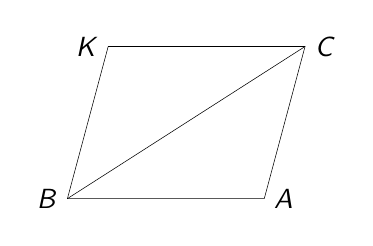
\begin{tikzpicture}
    \tkzDefPoints{0/0/B, 2.5/0/A}
    \tkzDefShiftPoint[B](75:2){K}
    \tkzDefShiftPoint[A](75:2){C}
    \tkzDrawPolygon(B,A,C,K)
    \tkzLabelPoints[left](B,K)
    \tkzLabelPoints[right](A,C)
    \tkzDrawSegment(B,C)
    \end{tikzpicture}

    \vfill 
    
    \item \textbf{Given:} $\overline{BA} \cong \overline{DA}, \, \overline{CA} \cong \overline{EA}$ \quad \textbf{Prove:} $\angle C \cong \angle E$ \newline\\

    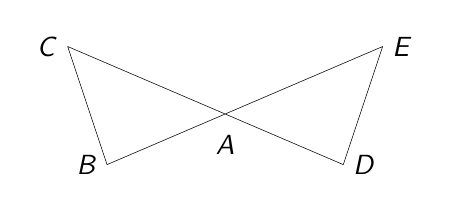
\begin{tikzpicture}
    \tkzDefPoints{0/0/A, -1.5/-0.5/B, 1.5/-0.5/D, -2/1/C, 2/1/E}
    \tkzDrawPolygon(B,E,D,C)
    \tkzLabelPoints[left](B,C)
    \tkzLabelPoints[below](A)
    \tkzLabelPoints[right](E,D)
    \end{tikzpicture}

    \vfill 

    \item \textbf{Given:} $\overline{AB} \cong \overline{AC}, \, M \text{is the midpoint of } \overline{BC}$    \quad \textbf{Prove:} $\angle AMB \cong \angle AMC$ \newline\\

    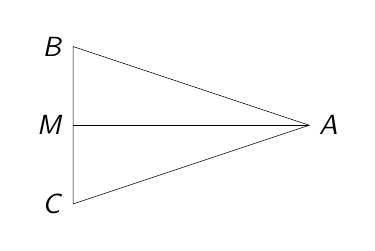
\begin{tikzpicture}
    \tkzDefPoints{0/0/A, -3/0/M, -3/1/B, -3/-1/C}
    \tkzLabelPoints[left](B,M,C)
    \tkzLabelPoints[right](A)
    \tkzDrawPolygon(A,B,C)
    \tkzDrawSegment(A,M)
    \end{tikzpicture}

    \vfill 
\end{enumerate}
\end{example}

\end{document}
